\newcommand{\Release}{}
\newcommand{\Slide}{}
\newcommand{\PrintLecture}{1}
\newcommand{\PrintSolution}{0}
\newcommand{\MyCourse}{データサイエンスコース}
\newcommand{\MySemester}{春}
\newcommand{\MySubject}{ビジネス アナリティクス}
\newcommand{\MyClass}{第17回ー分類}% フォルダ名自動挿入

%
% 科目共通定義
%

\newcommand{\OpenIntro}
{\MyRef{OpenIntro Statistics}{https://www.openintro.org/book/os}}

\newcommand{\R}{\textbf{R}}
\newcommand{\RStudio}{\textbf{RStudio}}
\newcommand{\Excel}{\textbf{Excel}}
\newcommand{\cs}[1]{\textcolor{blue}{\texttt{#1}}} % Console prompt >

\newcommand{\ra}{\rightarrow}
\newcommand{\Ra}{\Rightarrow}

% Expectation E[X]
\def\E#1{E\big[#1\big]}
\def\S{\sum_{i=1}^n}

\newcommand{\B}{\hat{\beta}}
\newcommand{\SUM}{\sum_{i=1}^n}  % Summention from i=1 to n
\newcommand{\NH}{$\mathit{H}_0$} % Null hypthesis
\newcommand{\AH}{$\mathit{H}_1$} % Alternative hypothesis
\newcommand{\T}{\texorpdfstring{$t$}{}}% Student's t
\newcommand{\overtext}[3][1.5]{
  \mathrel{\overset{#2}{\scalebox{#1}[1]{$#3$}}}
}
\newcommand{\iid}{\overtext[2]{iid}{\sim}}
\newcommand{\convdist}{\overtext[2]{d}{\rightarrow}}
\newcommand{\convprob}{\overtext[2]{p}{\rightarrow}}
\newcommand{\as}[2]{\quad \text{as}\quad #1 \rightarrow #2}

\input{../../tex/hss_lualatex.tex}
\input{../../tex/hss_moodle.tex}
\input{../../tex/hss_beamer.tex}

\begin{document}

\maketitle

\section{小テスト(\MyClass)}

\begin{quiz}{\MyClass}

\QuizMultipleChoices
{
  回帰分析の前提条件はどれか?
}
{
  \MyEnums
  {
    \item 等分散性(homoscedasticity; 誤差分散が一定)
    \item 正規性(normality; 誤差が正規分布に従う)
    \item 線形性(linearity; 説明変数と目的変数の関係は直線的)
    \item 独立性(independence; 説明変数が互いに独立)
  }
  回帰モデルを分析目的でなく予測目的で用いる時は独立性の条件は不要。
}
{10}
{*等分散性,正規性,線形性,独立性}
{ 等分散性,正規性,線形性,排反性}
{ 等分散性,標準性,線形性,独立性}
{ 等分散性,標準性,線形性,排反性}

\QuizMultipleChoices
{
   残差分析で,等分散性の確認に優れたグラフはどれか?
}
{
  尺度-位置グラフ(scale-location plot)
  \MyFig{0.45}{scale_location.png}
}
{20}
{ 残差 VS 適合値グラフ(residuals vs fitted plot)}
{*尺度-位置グラフ(scale-location plot)}
{ 残差 VS \ruby{梃子比}{てこひ}グラフ(residuals vs leverage plot)}
{ 正規Q-Qプロット(normal quantile-quantile plot)}

\QuizMultipleChoices
{
   残差分析で,予測値に与える影響の大きいデータの確認に優れたグラフはどれか?
}
{
  残差 VS \ruby{梃子比}{てこひ}グラフ(residuals vs leverage plot)
  \MyFig{0.9}{residuals_vs_leverage.png}
}
{20}
{ 残差 VS 適合値グラフ(residuals vs fitted plot)}
{ 尺度-位置グラフ(scale-location plot)}
{*残差 VS \ruby{梃子比}{てこひ}グラフ(residuals vs leverage plot)}
{ 正規Q-Qプロット(normal quantile-quantile plot)}

\QuizMultipleChoices
{
  \textbf{a}の分布のときの正規Q-Qプロットはどれか?
  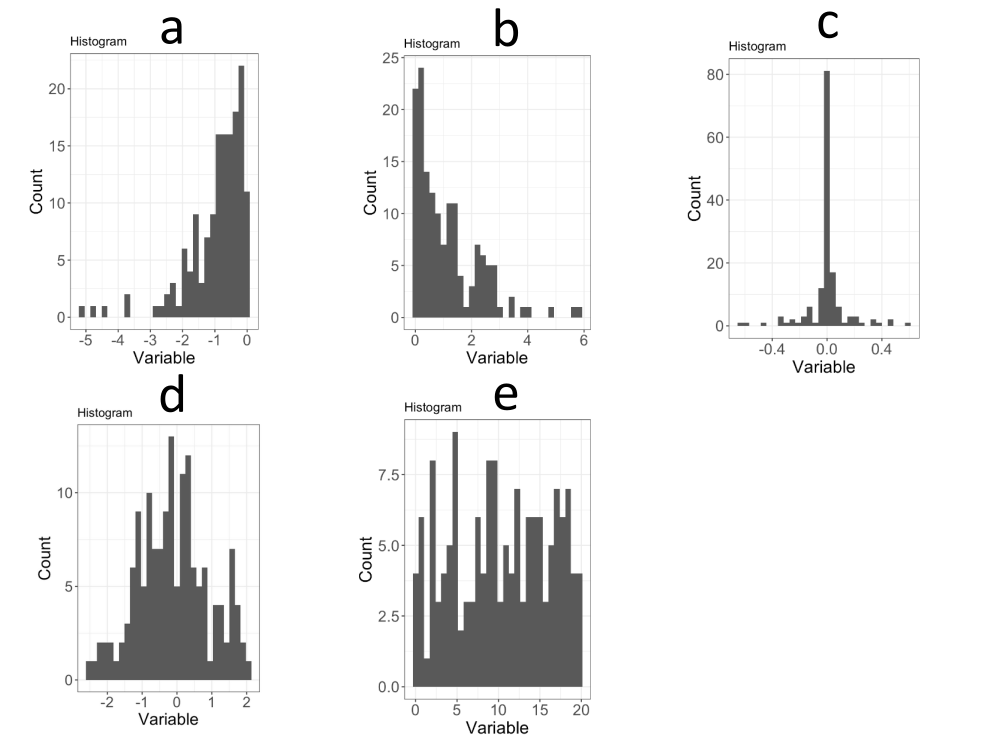
\includegraphics[width=0.45\textwidth]{quiz_qqplot_histogram.png}
  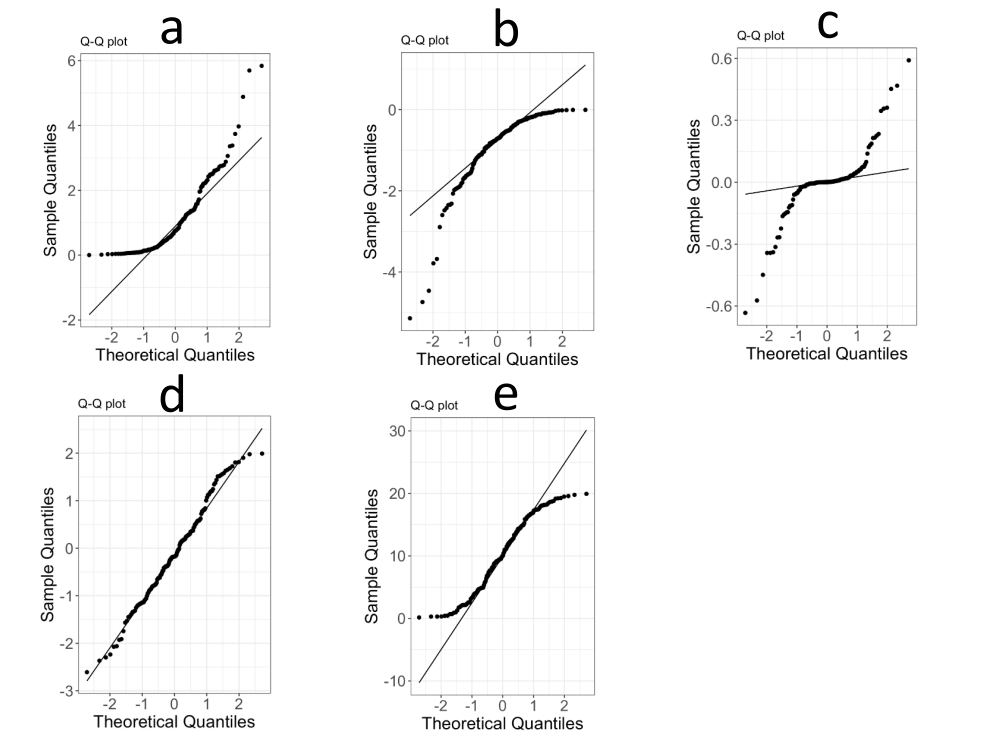
\includegraphics[width=0.45\textwidth]{quiz_qqplot.png}
}
{
  b
}
{10}
{ a}
{*b}
{ c}
{ d}

\QuizMultipleChoices
{
  \textbf{b}の分布のときの正規Q-Qプロットはどれか?
  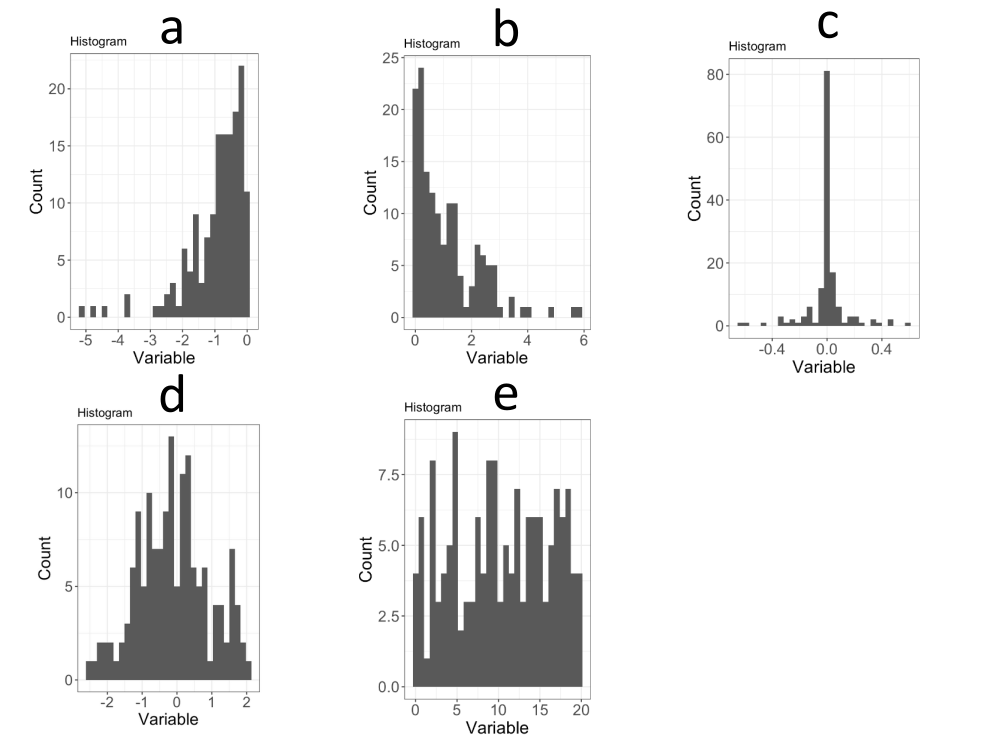
\includegraphics[width=0.45\textwidth]{quiz_qqplot_histogram.png}
  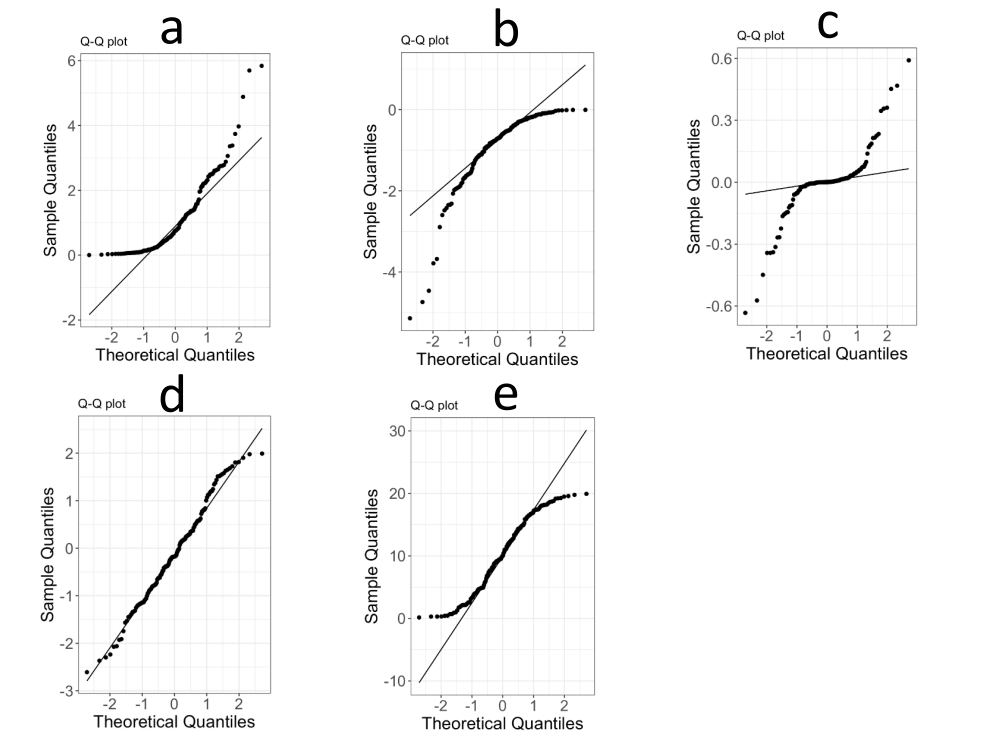
\includegraphics[width=0.45\textwidth]{quiz_qqplot.png}
}
{
  a
}
{10}
{*a}
{ b}
{ c}
{ e}

\QuizMultipleChoices
{
  \textbf{c}の分布のときの正規Q-Qプロットはどれか?
  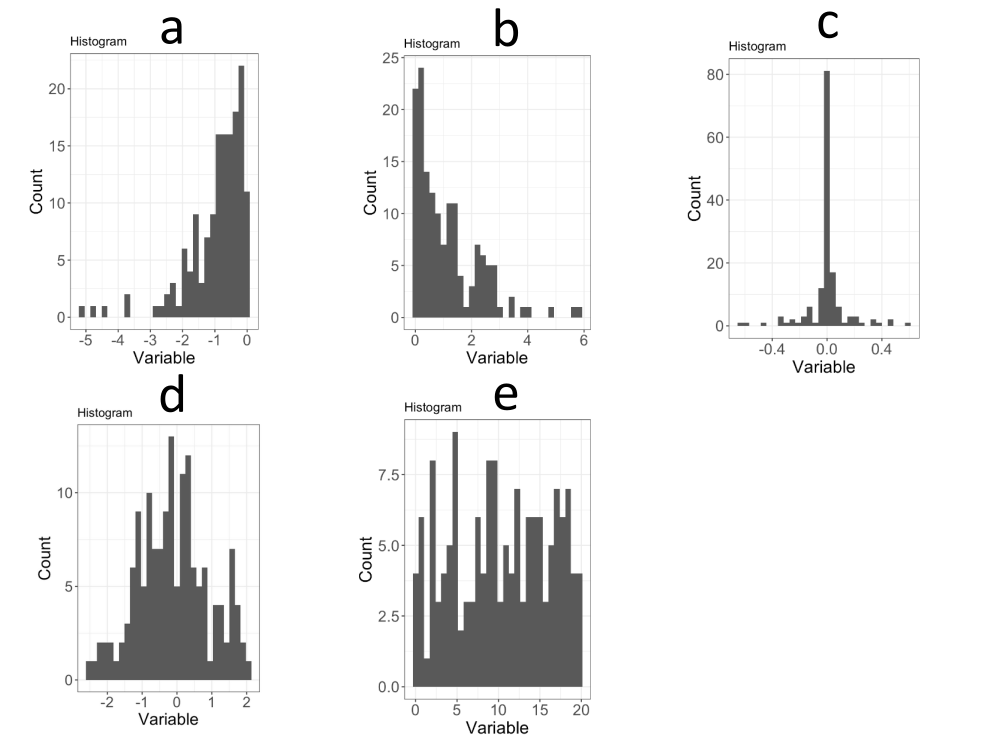
\includegraphics[width=0.45\textwidth]{quiz_qqplot_histogram.png}
  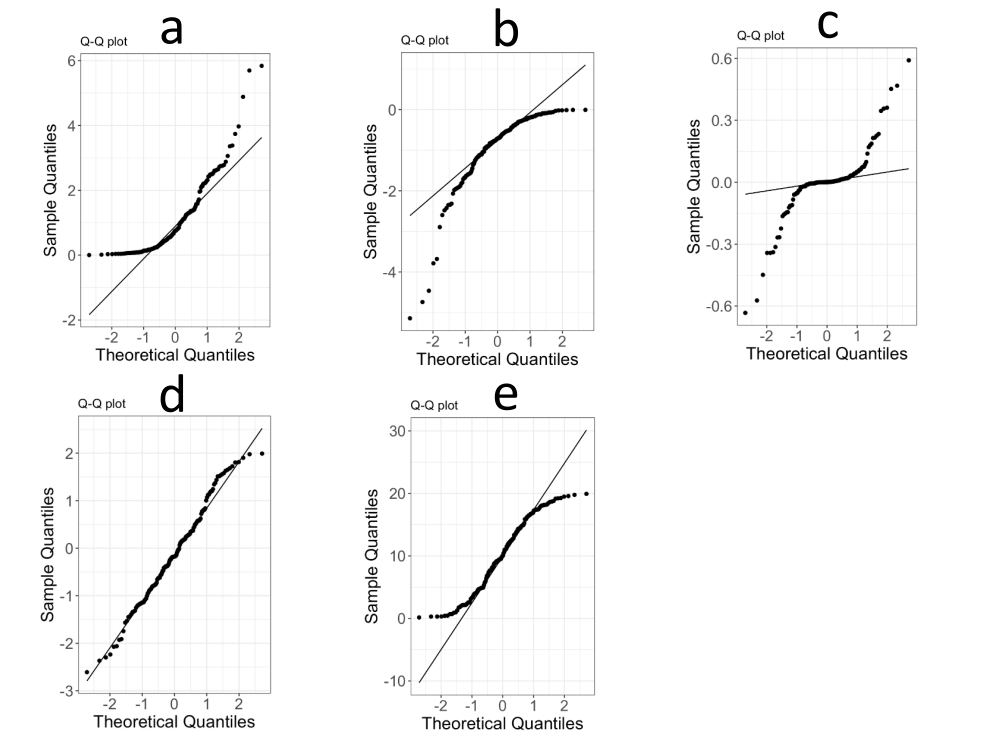
\includegraphics[width=0.45\textwidth]{quiz_qqplot.png}
}
{
  c
}
{10}
{ a}
{ b}
{*c}
{ d}

\QuizMultipleChoices
{
  \textbf{d}の分布のときの正規Q-Qプロットはどれか?
  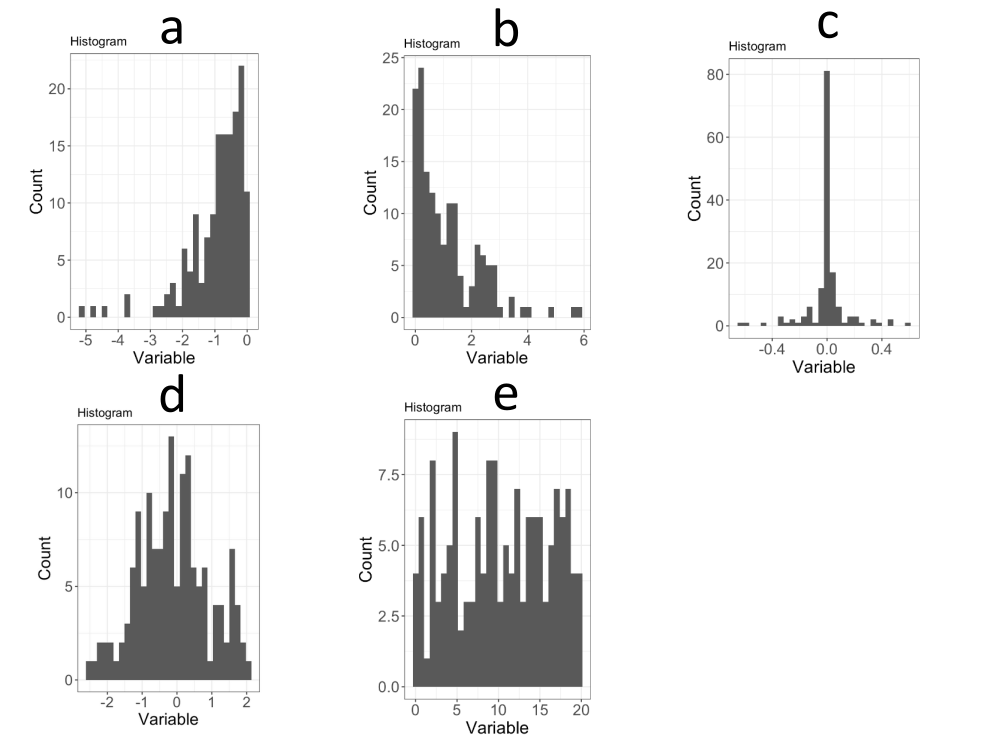
\includegraphics[width=0.45\textwidth]{quiz_qqplot_histogram.png}
  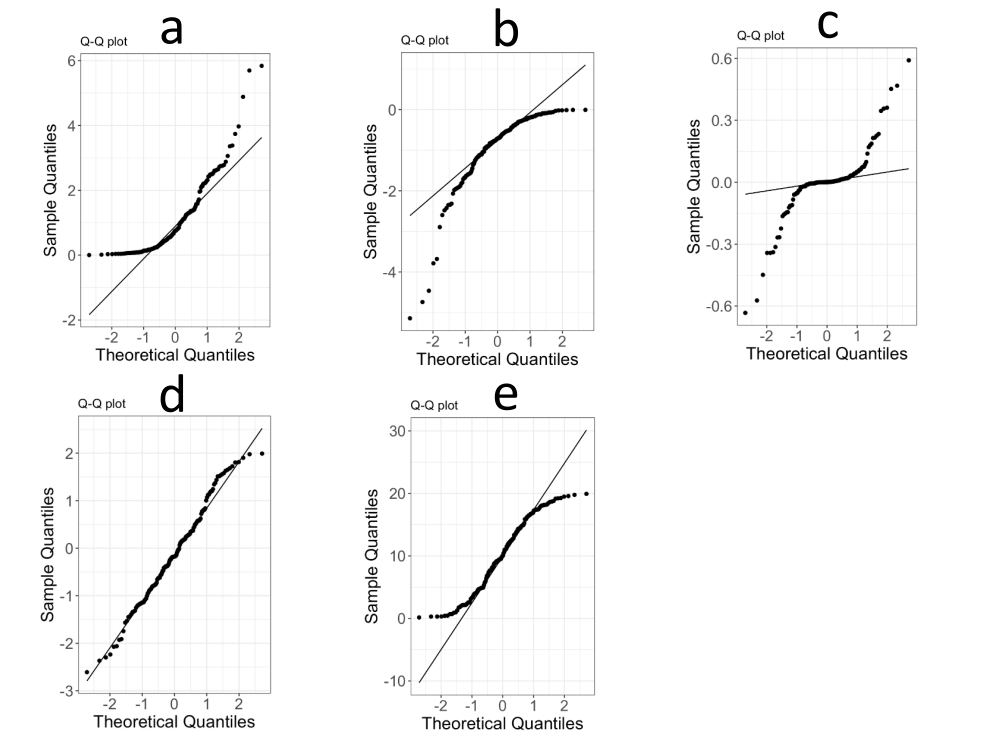
\includegraphics[width=0.45\textwidth]{quiz_qqplot.png}
}
{
  d
}
{10}
{ b}
{ c}
{*d}
{ e}

\QuizMultipleChoices
{
  \textbf{e}の分布のときの正規Q-Qプロットはどれか?
  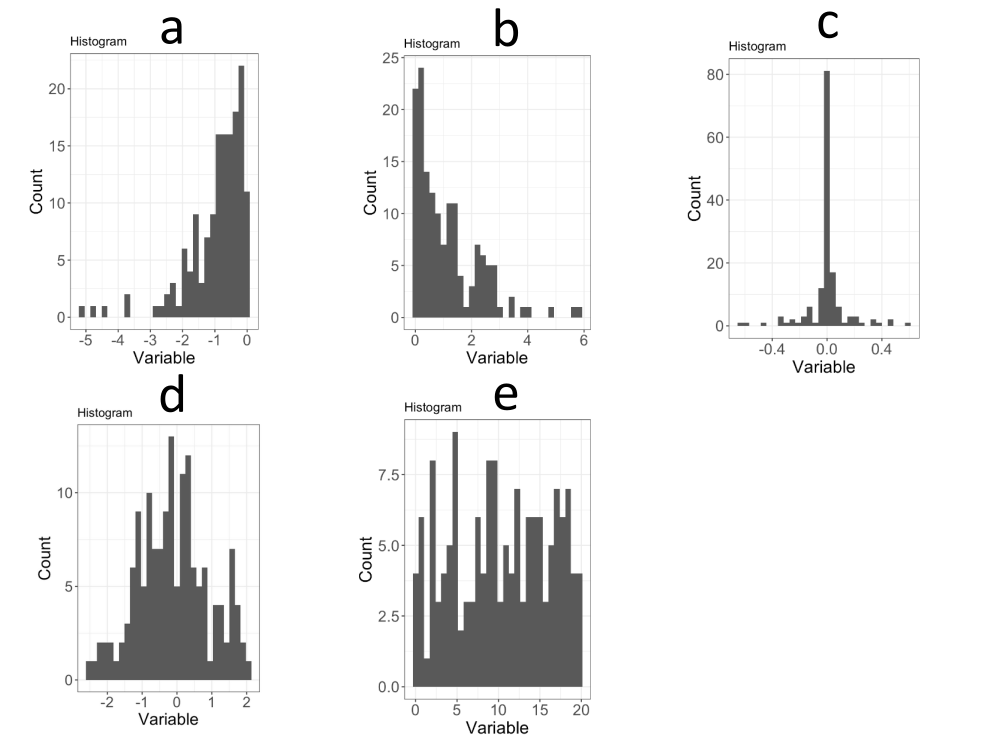
\includegraphics[width=0.45\textwidth]{quiz_qqplot_histogram.png}
  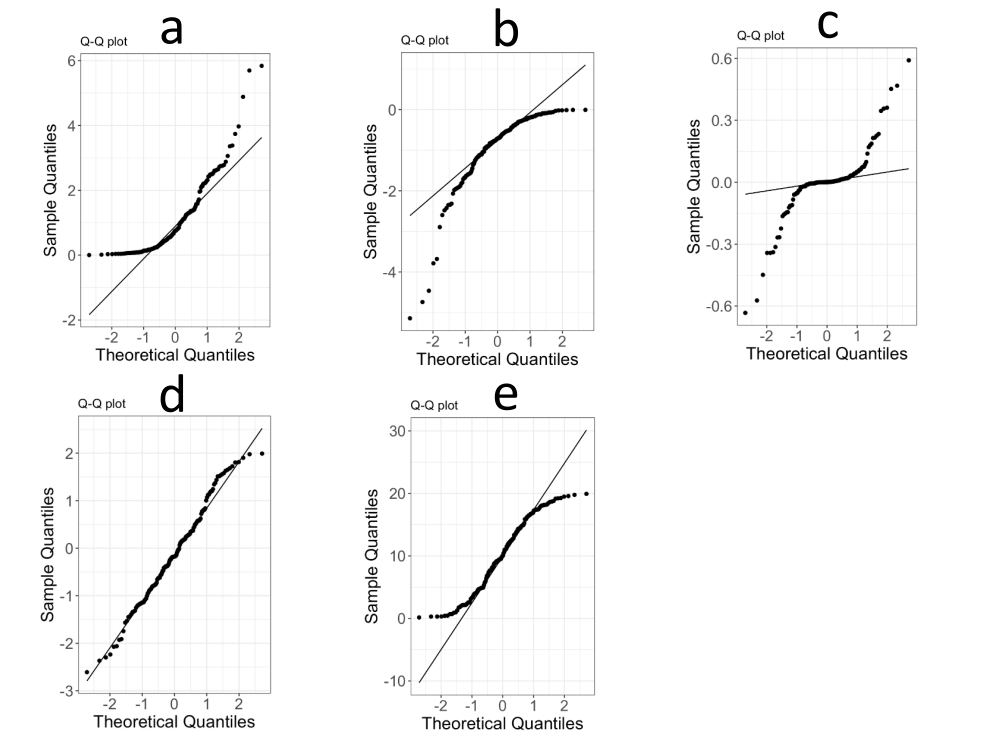
\includegraphics[width=0.45\textwidth]{quiz_qqplot.png}
}
{
  e
}
{10}
{ b}
{ c}
{ d}
{*e}

\end{quiz}

\end{document}
